%\VignetteIndexEntry{GAPS/CoGAPS Users Manual}
%\VignettePackage{CoGAPS}

\documentclass{report}
\usepackage{fullpage,./chicago,graphicx,subfigure,amssymb,amsmath,color,hyperref,underscore}

\author{Elana J. Fertig (\texttt{ejfertig@jhmi.edu}) and Michael F. Ochs (\texttt{ochsm@tcnj.edu})}
\title{GAPS/CoGAPS Users Manual}

\usepackage{Sweave}
\begin{document}
\Sconcordance{concordance:CoGAPSUsersManual.tex:CoGAPSUsersManual.Rnw:%
1 9 1 1 0 139 1 1 2 1 0 2 1 1 2 16 0 1 1 7 0 1 2 15 1 1 3 1 2 60 1 1 2 %
1 0 2 1 1 5 19 0 1 1 7 0 1 2 20 1 1 2 1 0 3 1 1 4 3 0 1 1 3 0 1 2 49 1 %
1 5 3 0 1 4 2 0 1 6 8 0 1 2 79 1 1 2 1 0 9 1 1 3 1 0 1 3 1 0 1 3 1 0 1 %
1 1 7 5 0 1 2 1 1 1 3 1 0 5 1 1 3 1 0 1 2 1 0 1 7 5 0 1 3 4 0 1 2 91 1}


\maketitle
\tableofcontents

\chapter{Introduction}

\par Gene Association in Pattern Sets (GAPS) infers underlying patterns in a matrix of measurements that can be interpreted as arising from the multiplication of two lower dimensional matrices.  The first development of this code in R/Biocondcutor was focused on gene expression analysis, however the original concept was used in spectral imaging.  The approach is a general form of matrix factorization using a stochastic algorithm.  In this vignette, we will focus on gene expression analysis for concreteness, but the factorization is applicable more broadly.

The Markov chain Monte Carlo (MCMC) matrix factorization that infers patterns also infers the extent to which individual genes belong to these patterns.  The CoGAPS algorithm extends GAPS to infer the coordinated activity in sets of genes for each of the inferred patterns based upon \cite{Ochs2009} and to refine gene set membership based upon \cite{Fertig2012}.

\par The GAPS algorithm is implemented in C++ and compiled and integrated into R using the Rcpp package.  GAPS is licensed under the GNU General Public License version 2.  You may freely modify and redistribute GAPS under certain conditions that are described in the top level source directory file \nolinkurl{COPYING}.

\par The R package CoGAPS is designed to facilitate the corresponding analysis of microarray measurements by calling the GAPS C++ library.  With the migration to C++ code, the installation as noted in Chapter \ref{install} should now be automatic.  Running instructions for the GAPS and CoGAPS analyses are provided in Sections \ref{GAPSRun} and \ref{CoGAPSRun}, respectively.  CoGAPS and GAPS are freely available at \url{https://github.com/ejfertig/CoGAPS} and through the CoGAPS Bioconductor package.

\par If you use the \texttt{CoGAPS} package for your analysis please cite:
\cite{Fertig2010} EJ Fertig, J Ding, AV Favorov, G Parmigiani, and MF Ochs (2010) CoGAPS: an R/C++ package to identify patterns and biological process activity in transcriptomic data. \textit{Bioinformatics} \textbf{26}: 2792-2793.

\par To cite the CoGAPS algorithm use:
\cite{Ochs2003} MF Ochs (2003) Bayesian Decomposition in \textit{The Analysis of Gene Expression Data: Methods and Software} G Parmigiani, E Garrett, R Irizarry, and S Zeger, ed. New York: Springer Verlag.

\par To cite the gene set statistic use:
\cite{Ochs2009} MF Ochs, L Rink, C Tarn, S Mburu, T Taguchi, B Eisenberg, and AK Godwin (2009) Detection of treatment-induced changes in signaling pathways in gastrointestinal stromal tumors using transcriptomic data. \textit{Cancer Research} \textbf{69}: 9125-9132.

\par To site the set-membership refinement statistic use:
\cite{Fertig2012} EJ Fertig, AV Favorov, and MF Ochs (2012) Identifying context-specific transcription factor targets from prior knowledge and gene expression data. \textit{2012 IEEE International Conference on Bioinformatics and Biomedicine}, B310, \textit{in press}.

\par To site GWCoGAPS or the PatternMarkers statistic use:
\cite{Stein-O’Brien2016} GL Stein-O’Brien, JL Carey, W Lee, M Considine, AV Favorov, E Flam, D Gaykalova, T Guo, L Li, T Sherman, S Sivy, R McKay, MF Ochs, C Colantuoni, and EJ Fertig (2016) PatternMarkers and Genome-Wide CoGAPS in Analysis in Parallel Sets (GWCoGAPS) for data-driven detection of novel biomarkers via whole transcriptome Non-negative matrix factorization (NMF). \textit{Bioinformatics} \textit{in press}.


\par Please contact Elana J. Fertig \url{ejfertig@jhmi.edu} or Michael F. Ochs \url{ochsm@tcnj.edu} for assistance.

\chapter{Installation Instructions} \label{install}

\par The GAPS, CoGAPS, and GWCoGAPS algorithms are implemented in an open source C++ software and an R package to facilitate analysis, visualization, and integration with other R tools (CoGAPS, available through Bioconductor).

\par With this version of CoGAPS, installation should be automatically completed through Bioconductor package installation:
\begin{verbatim}
source("http://www.bioconductor.org/biocLite.R")
biocLite("CoGAPS")
\end{verbatim}

\par The C++ software will be automatically compiled, linking to required boost libraries distributed as part of the CRAN \texttt{BH} package (\url{http://cran.r-project.org/web/packages/BH/index.html}) and Rcpp (\url{http://cran.r-project.org/web/packages/Rcpp/index.html}).

\chapter{Executing CoGAPS}

\par In this chapter, we describe how to run both the GAPS and CoGAPS algorithms.

\section{GAPS} \label{GAPSRun}

\par GAPS seeks a pattern matrix (${\bf{P}}$) and the corresponding distribution matrix of weights (${\bf{A}}$) whose product forms a mock data matrix (${\bf{M}}$) that represents the expression data ${\bf{D}}$ within noise limits ($\boldsymbol{\varepsilon}$).  That is,
\begin{equation}
{\bf{D}} = {\bf{M}} + \boldsymbol{\varepsilon} = {\bf{A}}{\bf{P}} + \boldsymbol{\varepsilon}.
\label{eq:matrixDecomp}
\end{equation}
The number of rows in ${\bf{P}}$ (columns in ${\bf{A}}$) defines the number of biological patterns that GAPS will infer from the measured microarray data or equivalently the number of nonorthogonal basis vectors required to span the data space.  As in the Bayesian Decomposition algorithm \cite{Ochs2006}, the matrices ${\bf{A}}$ and ${\bf{P}}$ in GAPS are assumed to have the atomic prior described in \cite{Sibisi1997}.  In the GAPS implementation, $\alpha_{A}$ and $\alpha_{P}$ are corresponding parameters for the expected number of atoms which map to each matrix element in ${\bf{A}}$ and ${\bf{P}}$, respectively.  The corresponding matrices ${\bf{A}}$ and ${\bf{P}}$ are found by MCMC sampling.

\subsection{Methods}

\par The GAPS algorithm is run by calling the \texttt{gapsRun} function in the CoGAPS R package as follows:
\begin{verbatim}
> gapsRun(D, S, ABins = data.frame(), PBins = data.frame(), nFactor = 7,
          simulation_id = "simulation", nEquil = 1000, nSample = 1000,
          nOutR = 1000, output_atomic = "FALSE", fixedBinProbs = "FALSE",
          fixedDomain = "N", sampleSnapshots = "TRUE", numSnapshots = 100,
          alphaA = 0.01, nMaxA = 1e+05, max_gibbmass_paraA = 100,
          alphaP = 0.01, nMaxP = 1e+05, max_gibbmass_paraP = 100)
\end{verbatim}


\par \noindent \textbf{\underline{Input Arguments}}
The inputs that must be set each time are only the data and standard deviation matrices, with all other inputs having default values.  However, in reality it is essential to set at least nFactor, nEquil, and nSample based on the expected dimensionality of the data and the number of iterations needed to explore the posterior distribution.  The arguments are as follows:
\begin{description}
\item[D]{The matrix of m genes by n samples of expression data.  The input should be a matrix object and row names and column names will be retained in the output matrices as appropriate.  }
\item[S]{The matrix of m genes by n samples of standard deviations for the expression data.  The values will be used in estimating the Likelihood, presently under an assumption of normal error distribution.}
\item[ABins]{a matrix of same size as A which gives relative probability of that element being non-zero (optional)}
\item[PBins]{a matrix of same size as P which gives relative probability of that element being non-zero (optional)}
\item[nFactor]{number of patterns (basis vectors, metagenes), which must be greater than or equal to the number of rows of FP }
\item[simulation_id]{name to attach to atoms files if created}
\item[nEquil]{number of iterations for burn-in}
\item[nSample]{number of iterations for sampling}
\item[nOutR]{how often to print status into R by iterations}
\item[output_atomic]{whether to write atom files (large)}
\item[fixedBinProbs]{Boolean for using relative probabilities given in Abins and Pbins}
\item[fixedDomain]{character to indicate whether A or P is domain for relative probabilities}
\item[sampleSnapshots]{Boolean to indicate whether to capture individual samples from Markov chain during sampling}
\item[numSnapshots]{the number of individual samples to capture}
\item[alphaA]{sparsity parameter for A domain}
\item[nMaxA]{PRESENTLY UNUSED, future = limit number of atoms}
\item[max_gibbmass_paraA]{limit truncated normal to max size}
\item[alphaP]{sparsity parameter for P domain}
\item[nMaxP]{PRESENTLY UNUSED, future = limit number of atoms}
\item[max_gibbmass_paraP]{limit truncated normal to max size}
\end{description}

The algorithm returns in the results a list with
\begin{description}
\item[Amean]{A matrix with the sampled mean value for the amplitude matrix ${{\bf{A}}}$.}
\item[Asd]{A matrix with the sampled standard deviation for the amplitude matrix ${{\bf{A}}}$.}
\item[Pmean]{A matrix with the sampled mean value for the pattern matrix ${\bf{P}}$.}
\item[Psd]{A matrix with the sampled standard deviation for the pattern matrix ${\bf{P}}$.}
\item[atomsAEquil]{A vector with the number of atoms in the A domain throughout the equilibration steps.}
\item[atomsASamp]{A vector with the number of atoms in the A domain throughout the sampling steps.}
\item[atomsPEquil]{A vector with the number of atoms in the P domain throughout the equilibration steps.}
\item[atomsPSamp]{A vector with the number of atoms in the P domain throughout the sampling steps.}
\item[chiSqValues]{A vector with the sample chi-squared values throughput sampling.}
\item[meanChi2]{${\chi^2}$ value of the final mean result, i.e. $\chi^2 = \frac{(D-AP)^2}{\sigma^2}$.}
\item[ASnapshots]{Samples of A matrices taken during sampling.}
\item[PSnapshots]{Samples of P matrices taken during sampling.}
\end{description}

\par Once the GAPS algorithm has been run, the inferred patterns and corresponding amplitude can be displayed using the \texttt{plotGAPS} function as follows:
\begin{verbatim}
> plotGAPS(Amean, Pmean, outputPDF="")
\end{verbatim}
where setting outputPDF to a string will redirect output to a PDF file from the screen.  The command
\begin{verbatim}
> plotP(Pmean,Psd)
\end{verbatim}
will create a plot of just the rows of the $mathbf{P}$ matrix with standard errors, which is equivalent to plotting the basis vectors for the matrix factorization.

\par \noindent \textbf{\underline{Input Arguments}}
\begin{description}
\item[Amean]{The amplitude matrix ${\bf{Amean}}$ obtained from GAPS.}
\item[Pmean]{The pattern matrix ${\bf{Pmean}}$ obtained from GAPS.}
\item[outputPDF]{Name of an \texttt{pdf} file to which the results will be output.  (Optional; default="" will output plots to the screen.)}
\item[Psd]{The standard deviation of the mean for ${\bf{Pmean}}$.}
\end{description}

\par \noindent \textbf{\underline{Side Effects}}
\begin{itemize}
  \item Save the plots of ${\bf{Amean}}$ and ${\bf{Pmean}}$ to the \texttt{pdf} file \texttt{outputPDF}.
\end{itemize}

\subsection{Example: Simple Simulation}

\par In this example, we have simulated data in SimpSim (\texttt{SimpSim.D}) with three known patterns (\texttt{SimpSim.P}) and corresponding amplitude (\texttt{SimpSim.A}) with specified activity in two gene sets (GSets).  In this data set, each gene set is overexpressed in one the simulated patterns and underexpressed in one.

\begin{Schunk}
\begin{Sinput}
> library('CoGAPS')
> data('SimpSim')
> nIter <- 5000
> results <- gapsRun(SimpSim.D, SimpSim.S, nFactor=3,
+ 		nEquil=nIter, nSample=nIter)
\end{Sinput}
\begin{Soutput}
Equil:1000 of 5000, Atoms:82(53)  Chi2 = 6903.69
Equil:2000 of 5000, Atoms:89(74)  Chi2 = 1557.9
Equil:3000 of 5000, Atoms:87(71)  Chi2 = 1481.69
Equil:4000 of 5000, Atoms:86(67)  Chi2 = 1511.34
Equil:5000 of 5000, Atoms:82(70)  Chi2 = 1492.74
Samp: 1000 of 5000, Atoms:76(71)  Chi2 = 1514.08
Samp: 2000 of 5000, Atoms:82(67)  Chi2 = 1499.49
Samp: 3000 of 5000, Atoms:79(66)  Chi2 = 1479.62
Samp: 4000 of 5000, Atoms:86(76)  Chi2 = 1482.75
Samp: 5000 of 5000, Atoms:73(81)  Chi2 = 1459.52
 *** Check value of final chi2: 1459.52 **** 
\end{Soutput}
\begin{Sinput}
> plotGAPS(results$Amean, results$Pmean, 'ModSimFigs')
\end{Sinput}
\begin{Soutput}
null device 
          1 
\end{Soutput}
\end{Schunk}
Figure \ref{fig:ModSim} shows the results from plotting the GAPS estimates of ${\bf{A}}$ and ${\bf{P}}$ using \texttt{plotGAPS}, which has a fit to ${\bf{D}}$ of $\chi^{2}=1381.45613920421$.
\begin{figure}[ht]
  \begin{center}
    \subfigure[Inferred amplitude matrix]{
      \includegraphics[width=0.45\linewidth]{ModSimFigs-Amplitude}
    }
    \subfigure[Inferred patterns]{
      \includegraphics[width=0.45\linewidth]{ModSimFigs-Patterns}
    }
  \end{center}
  \caption{Results from GAPS on simulated data set with known true patterns.}
  \label{fig:ModSim}
\end{figure}
Figure \ref{fig:ModSimPtrue} displays the true patterns used to create the SimpSim data, stored in \texttt{SimpSim.P}.
\begin{figure}[ht]
  \begin{center}
\includegraphics{CoGAPSUsersManual-ModSimPtrue}
  \end{center}
  \caption{Known true patterns used to generate SimpSim data.}
  \label{fig:ModSimPtrue}
\end{figure}

Figure \ref{fig:GS} shows the results from running CoGAPS on the SimpSim data.

\section{CoGAPS} \label{CoGAPSRun}

\par CoGAPS infers coordinated activity in gene sets active in each row of the pattern matrix ${\bf{P}}$ found by GAPS in a single step, by running both \texttt{GAPS} and then performing
the statistical analysis of \texttt{calcCoGAPSStat}.  Specifically, CoGAPS computes a $Z$-score based statistic on each column of the ${\bf{A}}$ matrix developed in \cite{Ochs2009}.  The resulting $Z$-score for pattern $p$ and gene set $i$, $\mathcal{G}_{i}$, with $G$ elements is given by
\begin{equation}
Z_{i,p} = \frac{1}{G} \sum\limits_{g \in \mathcal{G}_{i}} {\frac{{\bf{A}}_{gp}}{{\bf{Asd}}_{gp}}}
\label{eq:avgZ}
\end{equation}
where $g$ indexes the genes in the set and ${\bf{Asd}}_{gp}$ is the standard deviation of ${\bf{A}}_{gp}$ obtained from the MCMC sampling in GAPS.  CoGAPS then uses random sample tests to convert the Z-scores from eq. (\ref{eq:avgZ}) to $p$ values for each gene set.

\subsection{Methods}

\par The CoGAPS algorithm is run by calling the \texttt{CoGAPS} function in the CoGAPS R package as follows:
\begin{verbatim}
> results <- CoGAPS(data, unc, ABins = data.frame(), PBins = data.frame(),
                                   GStoGenes, nFactor = 7, simulation_id = "simulation",
                                   nEquil = 1000, nSample = 1000, nOutR = 1000,
                                   output_atomic = FALSE, fixedBinProbs = FALSE,
                                   fixedDomain = "N", sampleSnapshots = TRUE,
                                   numSnapshots = 100, plot = TRUE, nPerm = 500,
                                   alphaA = 0.01, nMaxA = 1e+05,
                                   max_gibbmass_paraA = 100, alphaP = 0.01,
                                   nMaxP = 1e+05, max_gibbmass_paraP = 100)

\end{verbatim}

\par \noindent \textbf{\underline{Input Arguments}}
\begin{description}
\item[$\ldots$]{Input arguments from GAPS.}
\item[GStoGenes]{List or data frame containing the genes in each gene set. If a list, gene set names are the list names and corresponding elements are the names of genes contained in each set. If a data frame, gene set names are in the first column and corresponding gene names are listed in rows beneath each gene set name.}
\item[nPerm]{Number of permutations used for the null distribution in the gene set statistic. (optional; default=500).}
\item[plot]{Use \texttt{plotGAPS} to plot results from the run of \texttt{GAPS} within \texttt{CoGAPS}.}
\end{description}

\par \noindent \textbf{\underline{List Items in Function Output}}
\begin{description}
\item[$\ldots$]{Output list from GAPS except vectors of sample atom numbers and individual $\chi^2$ values.}
\item[D]{The input data matrix.}
\item[Sigma]{The input standard deviation matrix.}
\item[GSUpreg]{p-values for upregulation of each gene set in each pattern.}
\item[GSDownreg]{p-values for downregulation of each gene set in each pattern.}
\item[GSActEst]{Conversion of p-values to activity estimates of each gene set in each pattern (see \cite{Ochs2009} for details on conversion.  Essentially values near $1$ indicate high activity for the set and near $-1$ indicate low activity.}
\end{description}

\par The CoGAPS algorithm can also be run manually by first running the GAPS algorithm described in Section \ref{GAPSRun} and then calling the function \texttt{calcCoGAPSStat} as follows:
\begin{verbatim}
> calcCoGAPSStat(Amean, Asd, GStoGenes, numPerm=500)
\end{verbatim}
The input arguments for \texttt{calcCoGAPSStat} are as described in the previous sections.  This function will output a list containing \texttt{GSUpreg}, \texttt{GSDownreg}, and \texttt{GSActEst}.

\subsection{Example: Simulated data}

\par In this example, we have simulated data in SimpSim with three known patterns (SimpSim.P) and corresponding amplitude (SimpSim.A) with specified activity in two gene sets (GSets).  In this data set, each gene set is overexpressed in two of the simulated patterns and underexpressed in one.

\begin{Schunk}
\begin{Sinput}
> library('CoGAPS')
> data('SimpSim')
> nIter <- 5000
> results <- CoGAPS(data=SimpSim.D, unc=SimpSim.S,
+ 		  GStoGenes=GSets,
+                   nFactor=3,
+                   nEquil=nIter, nSample=nIter,
+                   plot=FALSE)
\end{Sinput}
\begin{Soutput}
Equil:1000 of 5000, Atoms:77(54)  Chi2 = 1674.14
Equil:2000 of 5000, Atoms:76(59)  Chi2 = 1597.65
Equil:3000 of 5000, Atoms:77(62)  Chi2 = 1499.73
Equil:4000 of 5000, Atoms:85(76)  Chi2 = 1538.99
Equil:5000 of 5000, Atoms:89(58)  Chi2 = 1516.86
Samp: 1000 of 5000, Atoms:79(64)  Chi2 = 1496.5
Samp: 2000 of 5000, Atoms:65(64)  Chi2 = 1538.2
Samp: 3000 of 5000, Atoms:75(66)  Chi2 = 1539.65
Samp: 4000 of 5000, Atoms:72(71)  Chi2 = 1515.51
Samp: 5000 of 5000, Atoms:78(77)  Chi2 = 1496.59
 *** Check value of final chi2: 1496.59 **** 
\end{Soutput}
\begin{Sinput}
> plotGAPS(results$Amean, results$Pmean, 'GSFigs')
\end{Sinput}
\begin{Soutput}
null device 
          1 
\end{Soutput}
\end{Schunk}

Figure \ref{fig:GS2} shows the results from running CoGAPS on the GIST data in \cite{Ochs2009} with the option plot set to true.
\begin{figure}[ht]
\begin{center}
\subfigure[Inferred amplitude matrix]{
\includegraphics[width=0.45\linewidth]{GSFigs-Amplitude}
}
\subfigure[Inferred patterns]{
\includegraphics[width=0.45\linewidth]{GSFigs-Patterns}
}
\end{center}
\caption{Results from GAPS on data of simulated gene set data.}
\label{fig:GS2}
\end{figure}

\par Moreover, the gene set activity is provided in \texttt{results\$GSActEst} including p-values for upregulation in \texttt{results\$GSUpreg} and downregulation in \texttt{results\$GSDownreg}.

\subsection{Example: GIST Analysis}

\par We also provide the code that repeats the CoGAPS analysis of GIST data (GIST\_TS\_20084) with gene sets defined by transcription factors (TFGSList), as in the DESIDE analysis of \cite{Ochs2009}.  To minimize time in running the vignette, this is not done live.  However, running the code will complete the analysis and require on the order of an hour on a fast machine.

\begin{Schunk}
\begin{Sinput}
> library('CoGAPS')
> data('GIST_TS_20084')
> data('TFGSList')
> nIter <- 10000
> results <- CoGAPS(GIST.D, GIST.S, tf2ugFC,
+                   nFactor=5,
+                   nEquil=nIter, nSample=nIter,
+                   plot=FALSE)
> plotGAPS(results$Amean, results$Pmean, 'GISTFigs')
\end{Sinput}
\end{Schunk}

Figure \ref{fig:GS} shows the results from running CoGAPS on the GIST data in \cite{Ochs2009} with the option plot set to true.
\begin{figure}[ht]
\begin{center}
\subfigure[Inferred amplitude matrix]{
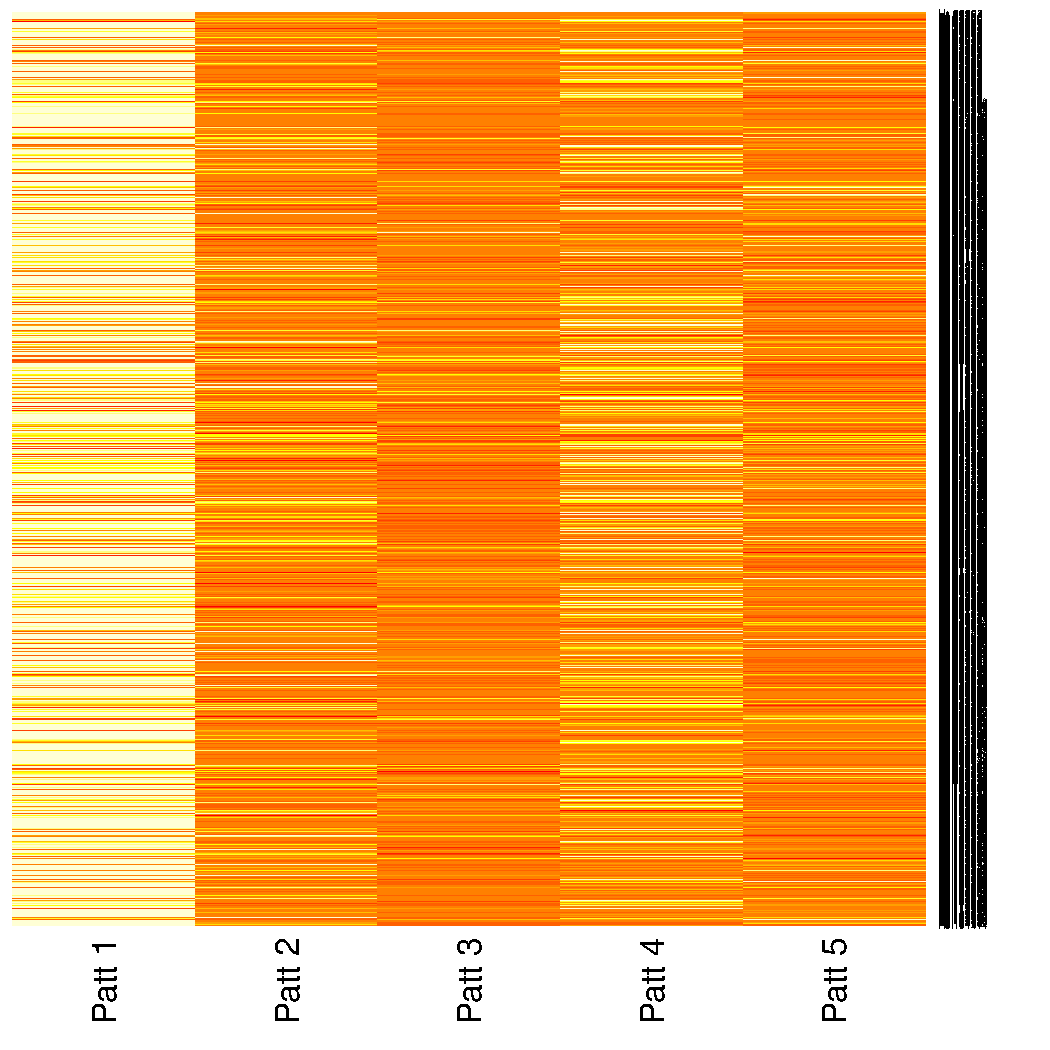
\includegraphics[width=0.45\linewidth]{GISTFigs-Amplitude}
}
\subfigure[Inferred patterns]{
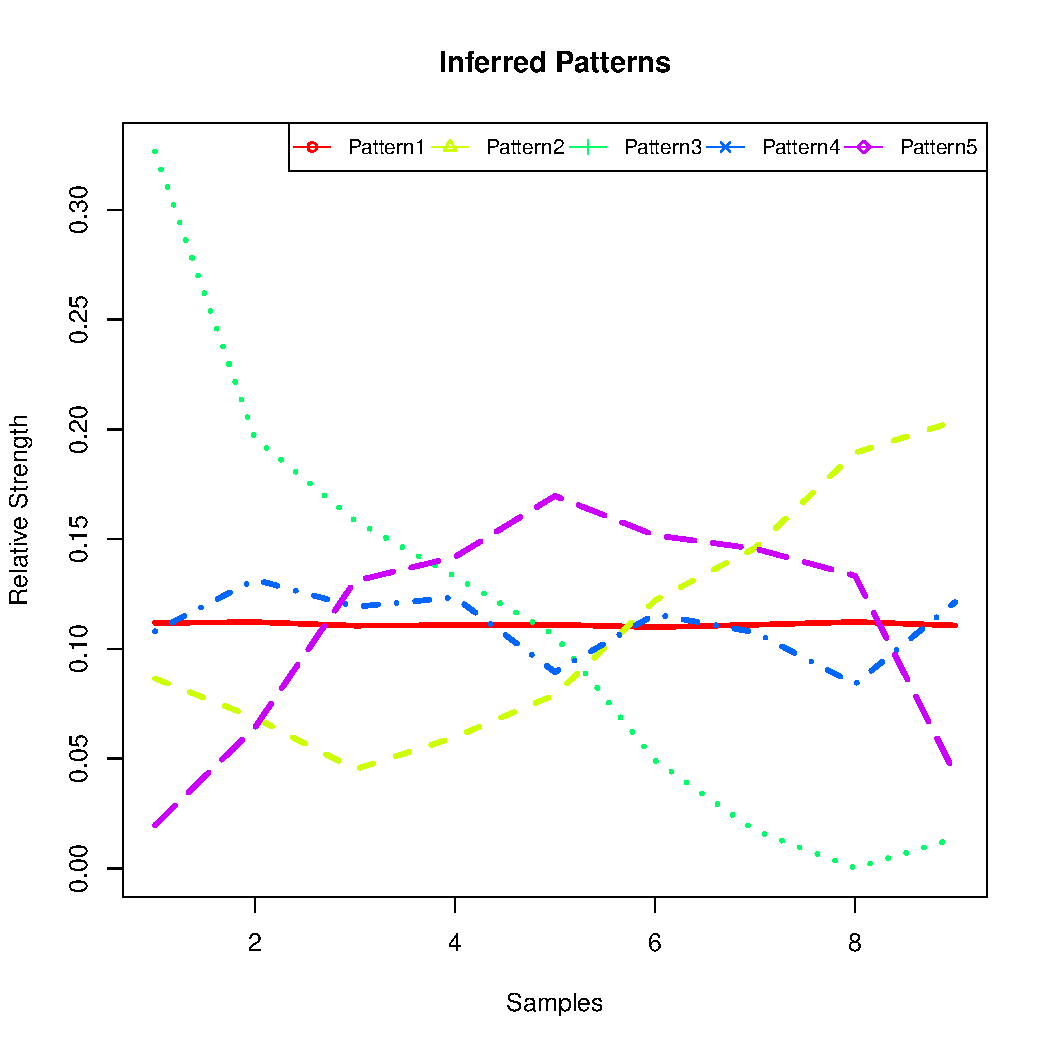
\includegraphics[width=0.45\linewidth]{GISTFigs-Patterns}
}
\end{center}
\caption{Results from GAPS on data of simulated gene set data.}
\label{fig:GS}
\end{figure}

\par Moreover, the gene set activity is provided in \texttt{results\$GSActEst} including p-values for upregulation in \texttt{results\$GSUpreg} and downregulation in \texttt{results\$GSDownreg}.

\section{Using CoGAPS-based statistics to infer gene membership in annotated gene sets}

\par As we describe in the previous section, the GAPS matrix factorization can be used to infer gene set activity in each pattern using the function \texttt{calcCoGAPSStat} \cite{Ochs2009}.  The \texttt{computeGeneGSProb} function extends this gene set statistic to compute a statistic quantifying the likely membership of each gene annotated to a set based upon its inferred activity \cite{Fertig2012}.  This statistic is formulated by comparing the expression pattern computed with CoGAPS of a given gene $g$ annotated as a member of $\mathcal{G}$ to the common expression pattern of all annotated members of $\mathcal{G}$.  This similarity is quantified with the following summary statistic
\begin{equation}
S_{g,\mathcal{G}} = \frac{\sum_{p} -log\left(\mbox{Pr}_{\mathcal{G}p}\right){\bf{A}}_{gp}/{\bf{Asd}}_{gp}}{\sum_{p} -log\left(\mbox{Pr}_{\mathcal{G}p}\right)},
\label{eq:summaryGSStat}
\end{equation}
where $\mbox{Pr}_{\mathcal{G}p}$ is the probability of upregulation of the geneset, returned from \texttt{calcCoGAPSStat} as \texttt{GSActEst} based upon eq.~(\ref{eq:avgZ}).  Similar to the gene set statistics, p-values for the set membership are computed with permutation tests that compare the value of $S_{g,\mathcal{G}}$ from eq.~(\ref{eq:summaryGSStat}) to the statistic formulated for a random gene set of the same size that also contains gene $g$.

\par The set membership statistic is computed from the results from the GAPS matrix factorization, computed with either the \texttt{GAPS} function described in Section \ref{GAPSR un} or the \texttt{CoGAPS} function described in Section \ref{CoGAPSRun} as follows:
\begin{verbatim}
> computeGeneGSProb(Amean, Asd, GStoGenes, numPerm=500)
\end{verbatim}

\par \noindent \textbf{\underline{Input Arguments}}
\begin{description}
\item[Amean]{Mean of the amplitude matrix estimated from the GAPS matrix factorization}
\item[Asd]{Standard deviation of the amplitude matrix estimated from the GAPS matrix factorization}
\item[GStoGenes]{List or data frame containing the genes in each gene set. If a list, gene set names are the list names and corresponding elements are the names of genes contained in each set. If a data frame, gene set names are in the first column and corresponding gene names are listed in rows beneath each gene set name.}
\item[nPerm]{Number of permutations used for the null distribution in the gene set and set membership statistics. (optional; default=500).}
\end{description}

\par \noindent \textbf{\underline{Function Output}}
\begin{description}
\item p-value of set membership for each gene specified in \texttt{GStoGenes}.
\end{description}

\subsection{Example on GIST Data}

\par Although not run in the interest of installation time, the following examples were used to generate some of the results in \cite{Fertig2012}, with the complete analysis code available from \url{http://astor.som.jhmi.edu/~ejfertig/ejfertig/Publications.html}.

\par This example refines transcription factor targets annotated in TRANSFAC (TFGSList) to identify context-specific targets from gene expression data (GIST\_TS\_20084)from \cite{Ochs2009}.

\begin{Schunk}
\begin{Sinput}
> # define transcription factors of interest based on Ochs et al. (2009)
> TFs <- c("c.Jun", 'NF.kappaB', 'Smad4', "STAT3", "Elk.1", "c.Myc", "E2F.1",
+          "AP.1", "CREB", "FOXO", "p53", "Sp1")
> # take the results from the previously run analysis
> # set membership statistics
> permTFStats <- list()
> for (tf in TFs) {
+      genes <- levels(tf2ugFC[,tf])
+      genes <- genes[2:length(genes)]
+      permTFStats[[tf]] <- computeGeneTFProb(Amean = results$Amean,
+                                             Asd = results$Asd, genes)
+ }
\end{Sinput}
\end{Schunk}


\chapter{Executing GWCoGAPS}

\par In this chapter, we describe how to run both the GWCoGAPS algorithm and a manual pipeline for genome wide NMF analysis.

\section{GWCoGAPS} \label{GWCoGAPS}

\subsection{Methods}
\par The GWCoGAPS algorithm is run by calling the \texttt{GWCoGAPS} function in the CoGAPS R package as follows:

\begin{verbatim}
> GWCoGAPS(D, S, nFactor, nSets, nCores = NA,
    saveBySetResults = FALSE, fname = ``'',
    PatternsMatchFN = patternMatch4Parallel,
    Cut = NA, minNS = NA, ...)
\end{verbatim}

\par \noindent \textbf{\underline{Input Arguments}}
The inputs that must be set each time are only the nSets, nFactor, and data and standard deviation matrices, with all other inputs having default values. Additional inputs to the gapsRun function, as outlined previously, can be used to taylor the analysis based on the expected dimensionality of the data. GWCoGAPS specific arguments are as follows:

\begin{description}
\item[D]{data matrix}
\item[S]{uncertainty matrix (std devs for chi-squared of Log Likelihood)}
\item[nFactor]{number of patterns (basis vectors, metagenes), which must be
greater than or equal to the number of rows of FP}
\item[nSets]{number of sets for parallelization}
\item[nCores]{number of cores for parallelization. If left to the default NA, nCores = nSets. }
\item[saveBySetResults]{logical indicating whether to save by intermediary by set results. Default is FALSE.}
\item[fname]{character string used to label file output. Default is "GWCoGAPS.out"}
\item[PatternsMatchFN]{function to use for pattern matching across sets. Default is patternMatch4Parallel.}
\item[Cut]{number of branches at which to cut dendrogram used in patternMatch4Parallel}
\item[minNS]{minimum of individual set contributions a cluster must contain used in patternMatch4Parallel}
\end{description}

\par Once the GWCoGAPS algorithm has been run, the inferred patterns and corresponding amplitudes can processed in the same way as output from gapsRun, gapsMapsRun, or CoGAPS.

\subsection{Example: Simulated data}

\par In this example, we use the same simulated data in SimpSim (SimpSim.D), as previously described, with three known patterns (SimpSim.P) and corresponding amplitude (SimpSim.A) with specified activity in two gene sets (GSets).

\begin{verbatim}
library(`CoGAPS')
data('SimpSim')
> GWCoGAPS(SimpSim.D, SimpSim.S, nFactor=3, nCores=NA, nSets=2,
            fname="test" ,PatternsMatchFN = postCoGAPSPatternMatch,
            sampleSnapshots = "TRUE", numSnapshots = 3)
> plotGAPS(AP.Fixed$A, AP.Fixed$P, 'ModSimFigs')
\end{verbatim}


\section{Manual Pipeline} \label{manpipe}

\par The functions that compose the core of the GWCoGAPS algorithm are also provided in the CoGAPS R package and can be used for a manual pipeline of the same analysis or to create a custom pipeline. Additionally, a web based shiny application is included for visualizing and editing the pattern matching process.

\subsection{PatternMatcher Shiny App}

\par \noindent \textbf{\underline{Input Arguments}}
The inputs that must be set each time is the PBySet. Additionally, the order and sample.color inputs are only available when calling patternMatcher in an interactive R session.

\begin{description}
\item[PBySet]{list of matched set solutions for the Pmatrix from an NMF algorithm}
\item[out]{optional name for saving output}
\item[order]{optional vector indicating order of samples for plotting. Default is NULL.}
\item[sample.color]{optional vector of colors of same lenght as colnames. Default is NULL.}
\end{description}

Figure \ref{fig:App1} shows a screenshot of the PatternMatcher Shiny App plotting the by-set results for pattern 1 generated from the simulated data as previously illustrated.
\begin{figure}[ht]
\begin{center}
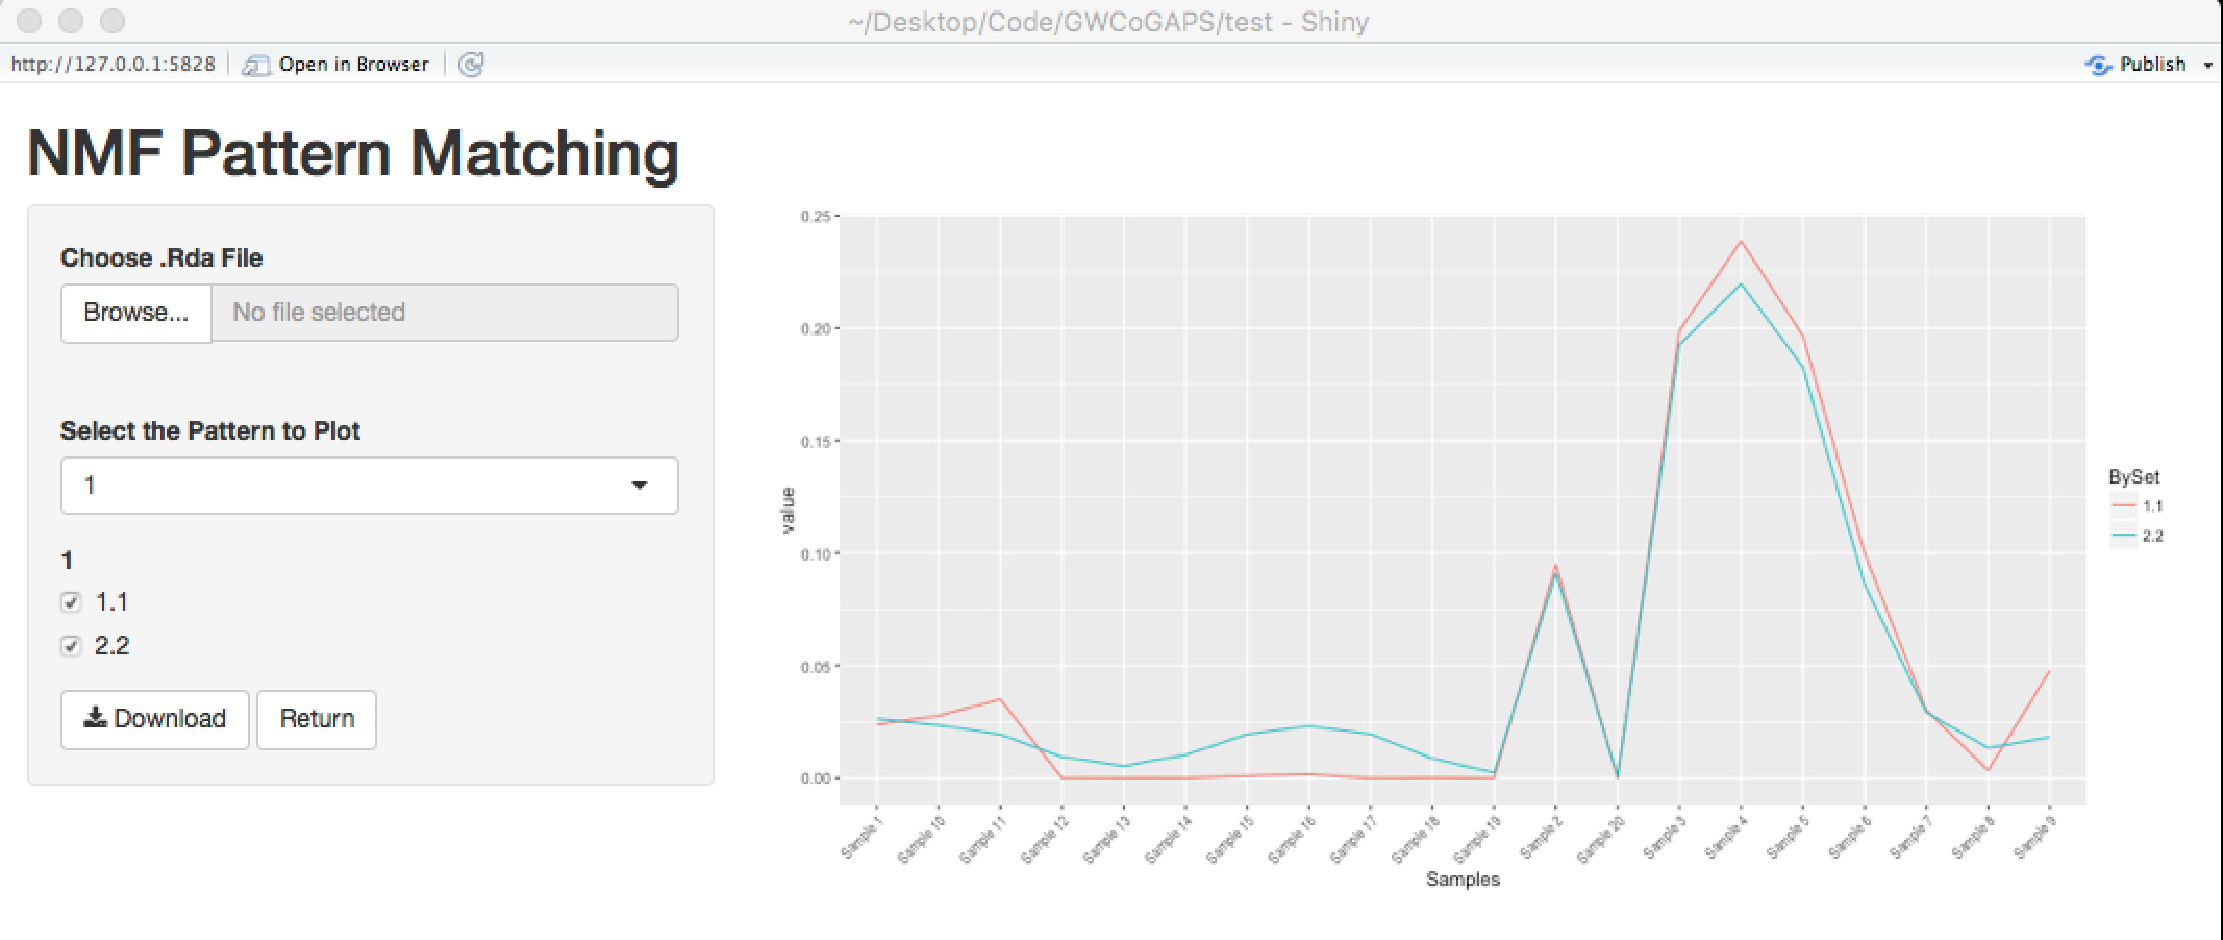
\includegraphics[width=0.95\linewidth]{ShinyApp}
\end{center}
\caption{Screenshot of shiny app for Pattern 1 of simulated data.}
\label{fig:App1}
\end{figure}

\subsection{Example: Simulated data}

\par This example will manually generate the same result as calling the \texttt{GWCoGAPS} function as given in the example in the previous section.

\begin{Schunk}
\begin{Sinput}
> data('SimpSim')
> D<-SimpSim.D
> S<-SimpSim.S
> nFactor=3
> nSets<-2
> nCores=NA
> numSnapshots=3
> saveBySetResults=TRUE
> fname="test"
> minNS=NA
> # break the data into sets
> genesInSets<-createGWCoGAPSSets(data=D, nSets=nSets, keep=FALSE)
> #generate seeds for parallelization
> nut<-generateSeeds(chains=nSets, seed=-1)
> # establish the number of cores that you are able to use
> if(is.na(nCores)){nCores<-nSets}
> registerDoParallel(cores=nCores)
> # run CoGAPS for each set
> AP <- foreach(i=1:nSets) %dopar% {
+   D <- as.matrix(D[genesInSets[[i]],])
+   S <- as.matrix(S[genesInSets[[i]],])
+   gapsRun(D=D, S=S, nFactor=nFactor,seed=nut[i],numSnapshots=numSnapshots)
+ }
> BySet<-reOrderBySet(AP=AP,nFactor=nFactor,nSets=nSets)
> matchedPs<-patternMatch4Parallel(Ptot=BySet$P,nP=nFactor,nS=nSets,cnt=nFactor,minNS=minNS,bySet=TRUE)
> # use shiny for pattern matching
> selectPBySet<-PatternMatcher(PBySet=matchedPs[["PBySet"]])
> library(reshape2)
> selectPBySet<-dcast(selectPBySet,  BySet ~ Samples)
> rownames(selectPBySet)<-selectPBySet$BySet
> selectPBySet<-as.matrix(selectPBySet[,-1])
> matchedPs<-patternMatch4Parallel(Ptot=selectPBySet,nP=nFactor,nS=nSets,cnt=nFactor,minNS=minNS,bySet=FALSE)
> #generate seeds for parallelization
> nut<-generateSeeds(chains=nSets, seed=-1)
> #final number of factors
> nFactorFinal<-dim(matchedPs)[1]
> # run fixed CoGAPS
> Fixed <- foreach(i=1:nSets) %dopar% {
+   D <- as.matrix(D[genesInSets[[i]],])
+   S <- as.matrix(S[genesInSets[[i]],])
+   AP <- gapsMapRun(D, S, FP=matchedPs, nFactor=nFactorFinal, fixedMatrix = "P",seed=nut[i],numSnapshots=numSnapshots)
+ }
> #extract A and Asds
> As4fixPs <- postFixed(AP.fixed=Fixed,setPs=matchedPs)
\end{Sinput}
\end{Schunk}


\chapter{PatternMarkers} \label{PatternMarkers}

\section{PatternMarkers}

\par The PatternMarkers statistic finds the genes most uniquely associated with a given pattern or linear combination of patterns by computing
\begin{equation}
\sqrt{\left(\bf{A}_{i}-l_{p}\right)^{\textit{t}} \left(\bf{A}_{i}-l_{p}\right)}
\label{eq:PatternMarkers}
\end{equation}
where  are the elements of the $\bf{A}$ matrix for the $\textit{i}^{th}$ gene scaled to have a maximum of one and \textit{l} is the $\textit{p}^{th}$ user specified norm. The genes are then ranked. In the case where \textit{l} is the identity vector, the ranking is run separately for each of the K patterns. Unique sets are generated by thresholding using the first gene to have a lower ranking, i.e. better fit to, another patterns.

\subsection{Methods}

\par The PatternMarkers statistic is run by calling the \texttt{patternMarkers} function in the CoGAPS R package as follows:

\begin{verbatim}
> patternMarkers(Amatrix = AP$Amean, scaledPmatrix = FALSE, Pmatrix = NA,
  threshold = "cut", lp = NA, full = FALSE, ...)
\end{verbatim}

\par \noindent \textbf{\underline{Input Arguments}}
\begin{description}
\item[Amatrix]{A matrix of genes by weights resulting from CoGAPS or other NMF decomposition}
\item[scaledPmatrix]{logical indicating whether the corresponding pattern matrix was fixed to have max 1 during decomposition}
\item[Pmatrix]{the corresponding Pmatrix (patterns X samples) for the provided Amatrix (genes x patterns). This must be supplied if scaledPmatrix is FALSE.}
\item[threshold]{the type of threshold to be used. The default "cut" will thresholding by the first gene to have a lower ranking, i.e. better fit to, a pattern. Alternatively, threshold="all" will return all of the genes in rank order for each pattern.}
\item[lp]{a vector of weights for each pattern to be used for finding markers. If NA markers for each pattern of the A matrix will be used.}
\item[full]{logical indicating whether to return the ranks of each gene for each pattern}
\end{description}

\par Once the PatternMarkers statistic has been run, a heatmap of each markers expression level can be displayed using the plotPatternMarkers function as follows:

\begin{verbatim}
> plotPatternMarkers(data = NA, patternMarkers = PatternMarkers,
      patternPalette = NA, sampleNames = NA, samplePalette = NA,
      colDenogram = TRUE, heatmapCol = "bluered", scale = "row", ...)
\end{verbatim}

\par \noindent \textbf{\underline{Input Arguments}}
\begin{description}
\item[data]{the dataset from which the patterns where generated}
\item[patternMarkers]{the list of genes generated from the patternMarkers function}
\item[patternPalette]{a vector indicating what color should be used for each pattern}
\item[sampleNames]{names of the samples to use for labeling }
\item[samplePalette]{a vector indicating what color should be used for each sample}
\end{description}

\subsection{Example: Simulated data}

\begin{verbatim}
# GWCoGAPS output
PatternMarkers<-patternMarkers(Amatrix=AP.fixed$A,scaledPmatrix=TRUE,threshold="cut")
plotPatternMarkers(data=D,patternMarkers=PatternMarkers,patternPalette=c("grey","navy","orange"))
# manual pipeline output
PatternMarkers<-patternMarkers(Amatrix=As4fixPs$A,scaledPmatrix=TRUE,threshold="cut")
plotPatternMarkers(data=D,patternMarkers=PatternMarkers,patternPalette=c("grey","navy","orange"))
\end{verbatim}

Figure \ref{fig:PM1} shows the results from running plotPatternMarkers on the PatternMarkers generated from the the GWCoGAPS and manual pipeline results generated from the simulated data as previously illustrated.
\begin{figure}[ht]
\begin{center}
\subfigure[GWCoGAPS Pattern Markers]{
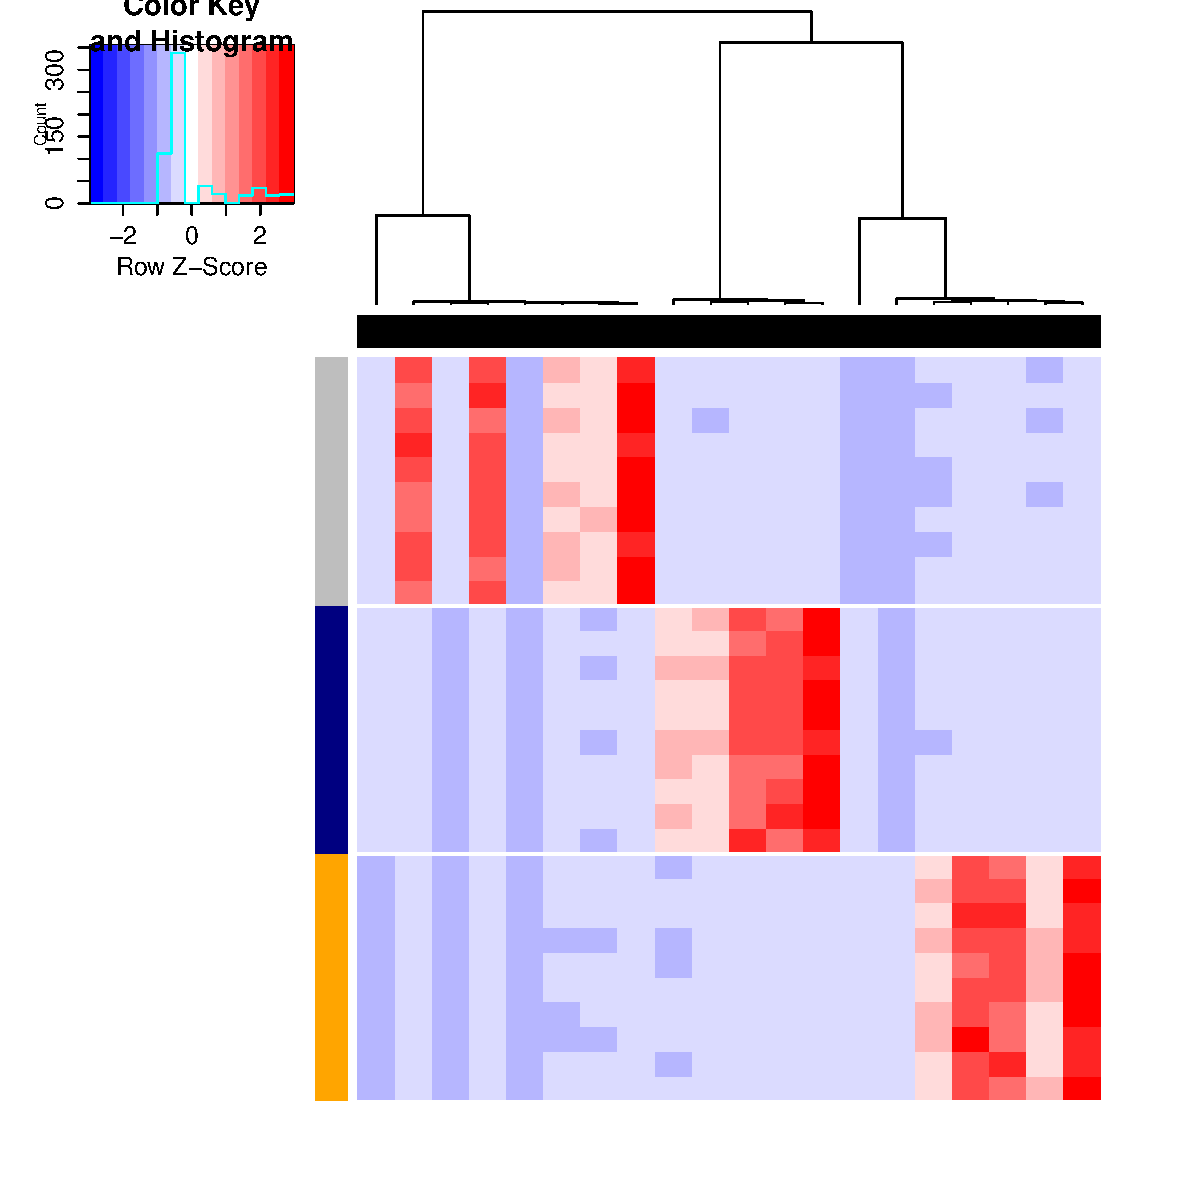
\includegraphics[width=0.45\linewidth]{GWCoGAPSPMs}
}
\subfigure[Pipeline Pattern Markers]{
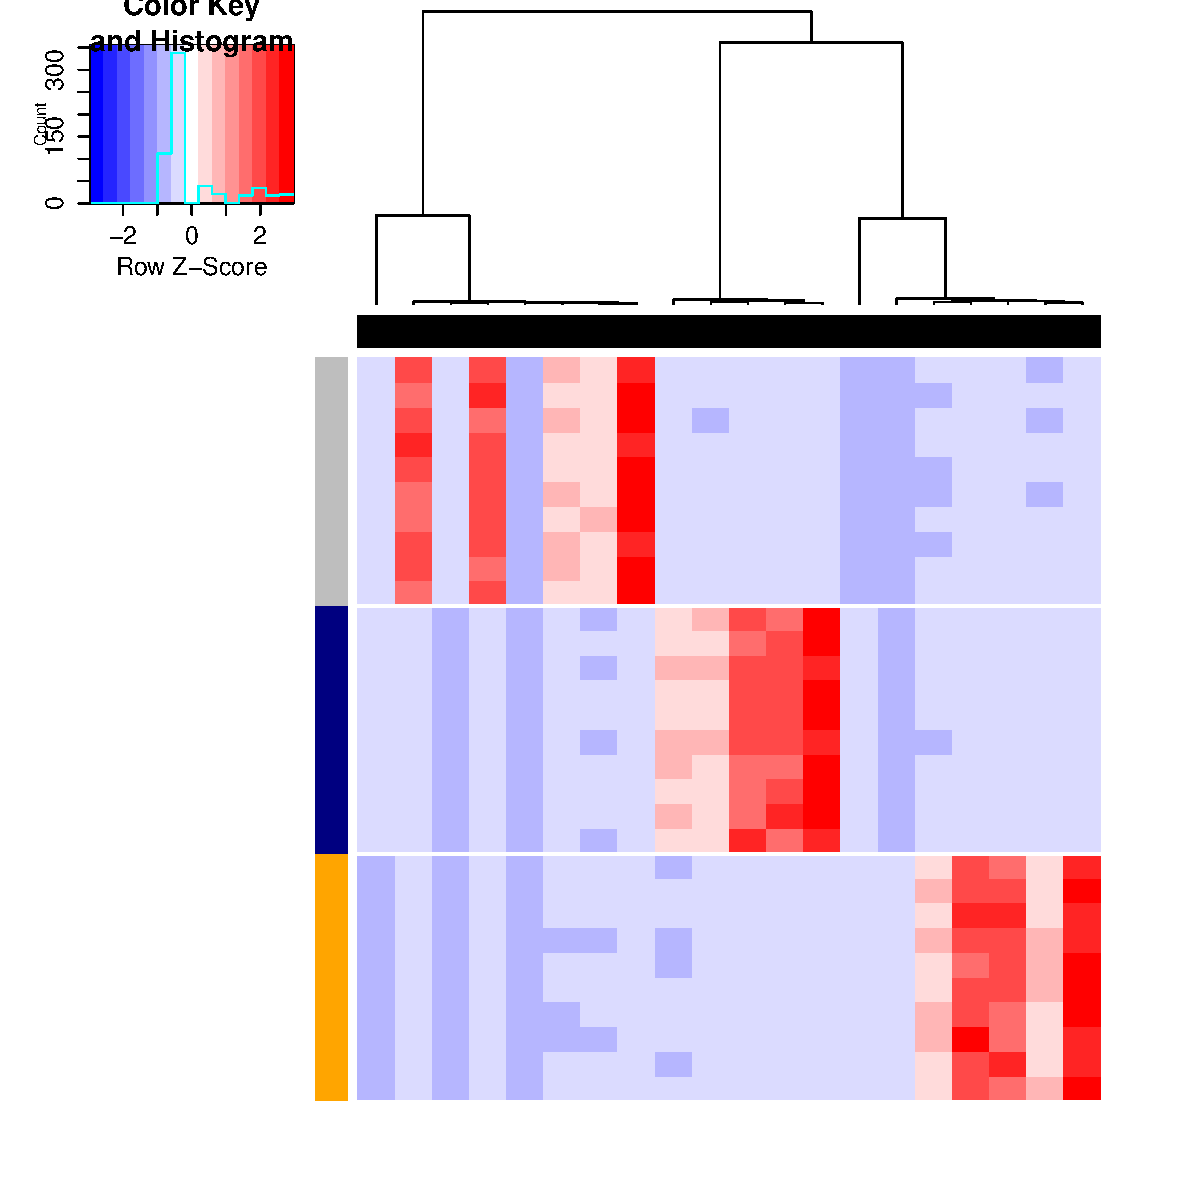
\includegraphics[width=0.45\linewidth]{ManPipePMs}
}
\end{center}
\caption{Heatmap of PatternMarkers expression levels for simulated data.}
\label{fig:PM1}
\end{figure}



\chapter{Feedback}

\par Please send feedback to Elana Fertig \texttt{ejfertig@jhmi.edu} or Michael Ochs \texttt{ochsm@tcnj.edu}.

\par If you want to send a bug report, please first try to reproduce the error.  The code is stochastic and we have seen many transient errors arising in the boost libraries which rarely repeat.  Send the data and please describe what you think should have happened, and what did happen.

\chapter{Acknowledgments}

\par This new version of CoGAPS relies on extensive recoding by Waishing Lee in C++ and work for C++ streamlining and R integration by Ondrej Maxian and Conor Kelton.  John Stansfield provided additional R code for visualization. Special thanks to paper co-authors Jie Ding, Alexander V. Favorov, and Giovanni Parmigiani for statistical advice in developing the GAPS / CoGAPS algorithms.  Additional thanks to Simina M. Boca, Ludmila V. Danilova, Genevieve Stein-O'Brien, Jeffrey Leek, and Svitlana Tyekcheva for their useful feedback.

\par This work was funded by NIH/NLM R21LM009382, NIH/NLM R01LM011000, NIH/NCI K25CA141053, and NSF Grant 0342111.

\bibliographystyle{plain}
\bibliography{AppNote}

\end{document}
